\section{The Ethereum angle}\label{sec:eth}

This section separates what exists from what is a direction. Nothing in it describes a shipped product for machine attestation on Ethereum. It is shorter than in 0.9.2, because the kernel repository holds no Solidity and nothing in this release moved the direction forward. We keep it because the question is why the project started, and because the box of Section~\ref{sec:box} sharpens it.

\subsection{The weak link}

Ethereum secures its state with consensus and with code that every node executes. The machines at its edges are outside that guarantee. A wallet machine that runs a compromised program can sign whatever the program asks. A validator's signing key is only as safe as the server that holds it. An RPC provider sees which accounts a given network address asks about, and that links a person's location to their holdings. A contract can check a signature. It cannot learn anything about the machine that produced it.

The box adds a smaller point. A wallet that reads a seed from a file is only as private as every program that can read that file. In \nonos{} a program in a box has no access to the person's files at all. That is a property of the endpoint, and no on-chain rule can see it.

\subsection{What exists today}

\begin{figure}[t]
\centering
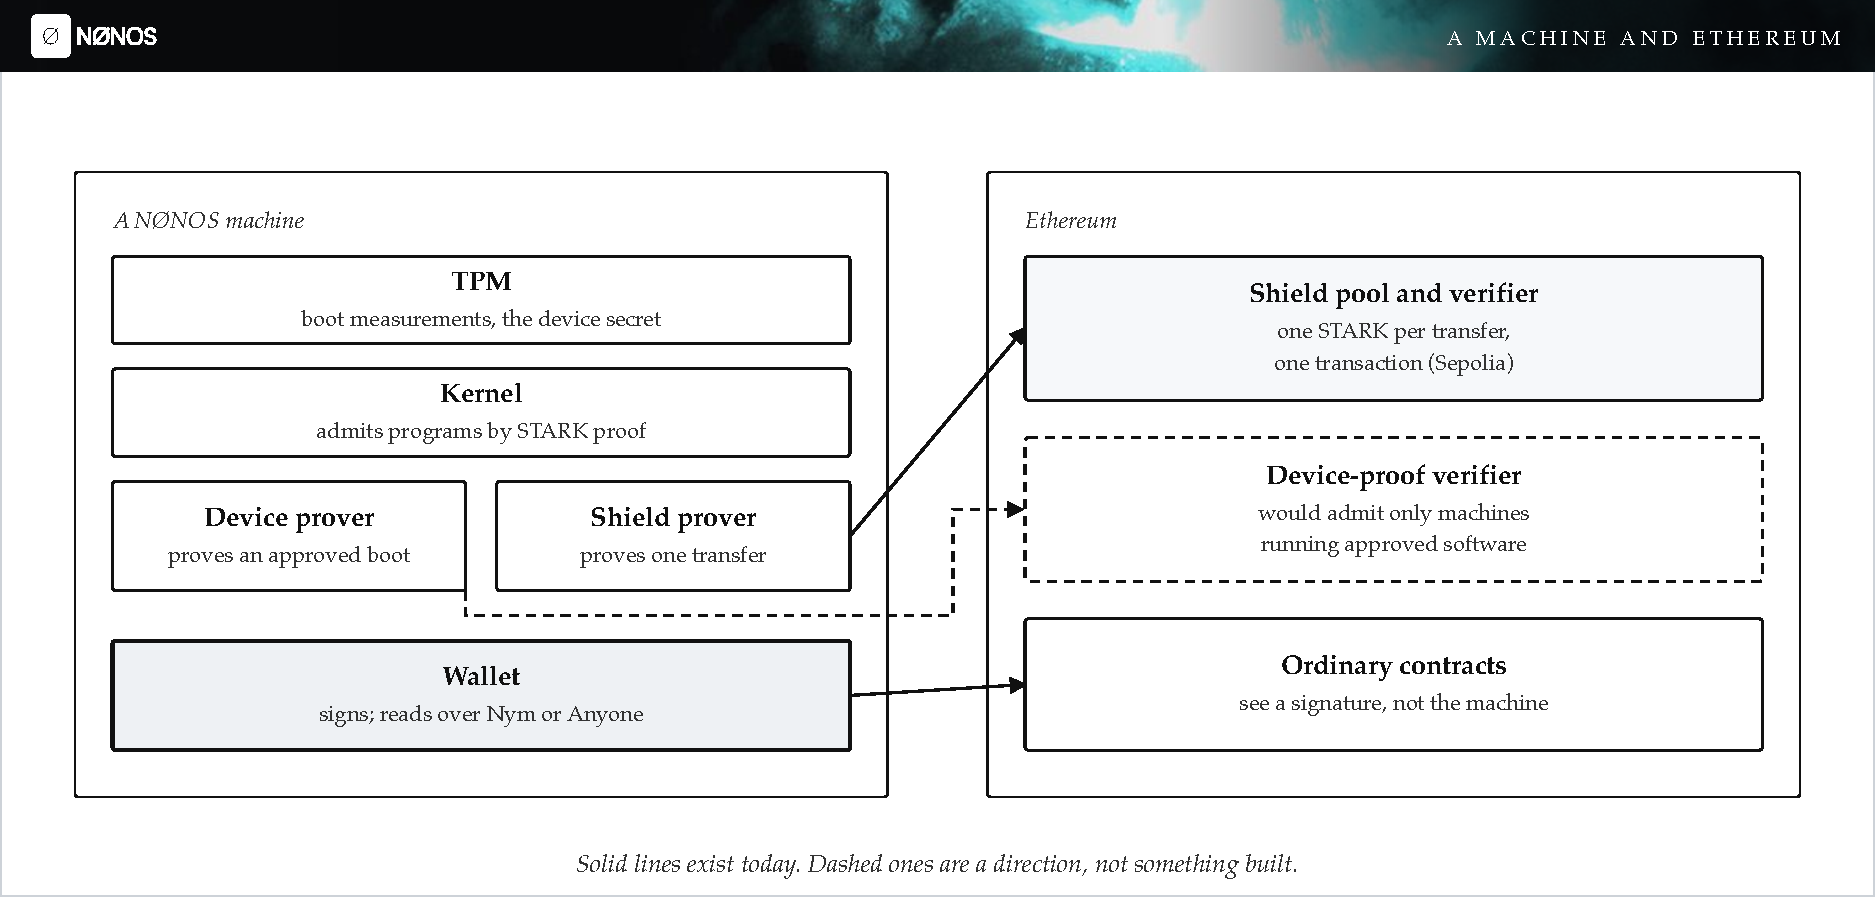
\includegraphics[width=0.84\textwidth]{figures/diagram-machine-and-ethereum.pdf}
\caption{What connects a \nonos{} machine to Ethereum, and what does not exist yet. Solid lines exist today; dashed ones are a direction, not something built. Sources: \code{docs/security/stark-attestation.md}, \code{nonos-device-attest/README.md}, \code{abi/NOX\_CONTRACTS.md}.}
\label{fig:eth}
\end{figure}

A \nonos{} machine can produce proofs about itself. Three artefacts exist, all checked off-chain. The admission proofs: every enrolled kernel, loader and capsule carries a STARK of membership under a public root. The TPM quote from \code{MkAttestDoc}, which names the machine and is withheld from any capsule with network rights. And the anonymous device proof of Section~\ref{sec:chain}, whose own README lists it as built and never run on a booted image, and which no verifier service or contract consumes.\srcs{docs/security/stark-attestation.md}{nonos-device-attest/README.md}

The wallet hides the RPC link. The wallet's chain reads go over Nym or Anyone, with host names resolved at the exit, and never over Direct (Section~\ref{sec:net}).

The NOX token has a contract set specified in the tree. \code{abi/NOX\_CONTRACTS.md} describes a contributor-reward system: off-chain receipts for work such as boots and capsule builds, aggregated into Merkle roots and paid from reward pools, with a deployment record on Ethereum mainnet under a 3-of-5 Safe. We did not query the chain to confirm the deployment, and the Solidity is not in this repository. The page is explicit that "v1 verification is off-chain with open tooling" and that v1 does no on-chain ZK verification. In 0.9.2 the same page listed ten contracts; it now lists eight, and we report it as the document stands.\srcs{abi/NOX_CONTRACTS.md}{abi/nox_deployment.json}

The Shield pool, which settles a private transfer with one STARK checked by a verifier contract, is described in a separate paper \cite{shield} and in repositories that are not part of this tree. We cite it and make no claim about it that we checked here. Its authors state that it has not been audited.

\subsection{What does not exist}

No contract verifies anything about a machine. No deployed contract checks an admission proof, a TPM quote or a device proof, and no transaction signature produced on \nonos{} is bound to an attested state. The project's public plan lists attested clients as an on-chain fact under work it is not building.\src{https://nonos.software/roadmap/}

\subsection{The direction}

The pieces suggest a path to a machine that proves to a contract what it runs. We state the steps and what each would need, without claiming any.

\begin{enumerate}
\item A verifier contract for the device proof. It proves a different statement over a different trace from the Shield pool's, so it would be a new contract with its own gas cost and its own audit.
\item Roots on chain: the release's bootloader, kernel and device-registry roots, from a source a contract trusts, such as a registry updated by the release's multisig.
\item Scope and freshness. The statement already binds a verifier scope and a nonce and yields one tag per device per scope, so a contract could use its own address as the scope and a recent block hash as the nonce.
\item Binding an action to the proof. The statement has no field for a public key or a message, so letting a contract accept a signature only from an attested machine would change the circuit.
\end{enumerate}

Two limits would remain. The proof shows that an approved chain exists and that the prover holds an enrolled device secret; that this machine booted that chain rests on the TPM releasing the secret only in that boot state, and so on the TPM and firmware being honest. And the proof says nothing about the behaviour of the code it admits, only its identity. Section~\ref{sec:box} is the other half of that sentence: identity of the system's own code from the proof, behaviour of everyone else's from the box. A contract that wanted to know that the signing machine could not be reached by a stray program would need both.
